%\documentclass[12pt, draftclsnofoot, onecolumn]{IEEEtran}
\documentclass[journal]{IEEEtran}
\usepackage{etex}
\reserveinserts{100}
%\usepackage{spconf}
\usepackage{mathtools}
\usepackage[dvipsnames]{xcolor}
\usepackage{graphics, theorem, times, amsfonts, graphicx, amssymb, cite}
\usepackage[outdir=./]{epstopdf}
\usepackage{tikz}
%\usepackage{fix2col}
\usetikzlibrary{shapes,arrows}
\usetikzlibrary{matrix} % for block alignment
\usetikzlibrary{decorations.markings} % for arrow heads
\usetikzlibrary{calc} % for manimulation of coordinates
\usetikzlibrary{decorations.pathmorphing,snakes, positioning, decorations.pathreplacing}

\usetikzlibrary{fit}
%\input{figures/tikh_styles}
\usepackage{pgfplots}
\usepackage{color}
\usepackage{setspace}
\usepackage{hyperref}
\usepackage{multirow}
\usepackage{rotating}
\usepackage{comment}
%\usepackage{flushend}
\usepackage{caption}
\usepackage{subcaption}
\usepackage[affil-it]{authblk}
\usepackage{bm}
\usepackage{algorithm}
\usepackage{algorithmic}
\usepackage{enumerate}
\usepackage{morefloats}
\usepackage{setspace}

\input{../mysymbol.sty}
\input{../my_sections}
\input{../TikZGallery-master/Sty/TikZGallery-Preamble}
%\renewcommand{\baselinestretch}{.995}
\newcommand{\QED}{\hfill\ensuremath{\blacksquare}}
\newcommand{\norm}[1]{\ensuremath{\left\| #1 \right\|}}

\def \vneg {\vspace{-2cm}}

\def\whp{\text{w.h.p}}
\def\E{\mathbb{E}}
\def\P{\mathbb{P}}
\def\supp{\text{support}}
\def\Tr{\text{Tr}}

\def\keywords{
{\bfseries\textit{Index Terms}---\,\relax%
}}
\def\endkeywords{\par}

%\addtolength{\textwidth}{10mm}
%\addtolength{\evensidemargin}{-5mm}
%\addtolength{\oddsidemargin}{-5mm}
%\addtolength{\textheight}{10mm}
%\addtolength{\topmargin}{-5mm}

%\renewcommand \blue[1]{}  \renewcommand \red[1]{

\newtheorem{assumption}{\hspace{0pt}\bf Assumption}
\newtheorem{lemma}{\hspace{0pt}\bf Lemma}
\newtheorem{proposition}{\hspace{0pt}\bf Proposition}
\newtheorem{example}{\hspace{0pt}\bf Example}
\newtheorem{observation}{\hspace{0pt}\bf Observation}
\newtheorem{theorem}{\hspace{0pt}\bf Theorem}
\newtheorem{corollary}{\hspace{0pt}\bf Corollary}
\newtheorem{fact}{\hspace{0pt}\bf Fact}
\newtheorem{remark}{\hspace{0pt}\bf Remark}
\newtheorem{test}{\hspace{0pt}\it Test Case}
\newtheorem{definition}{\hspace{0pt}\bf Definition}
\newtheorem{conj}{\hspace{0pt}\bf Conjecture}
\newtheorem{method}{\hspace{0pt}\bf Method}


% Title.
% ------

\title{Control Aware Radio Resource Allocation in Low Latency Wireless Control Systems}
%
% Single address.
% ---------------

\author{Mark Eisen$^*$ \quad Mohammad M. Rashid$^\dagger$ \quad Konstantinos Gatsis$^*$ \\ \textup{Dave Cavalcanti$^\dagger$\quad Nageen Himayat$^{\dagger}$ \quad Alejandro Ribeiro$^*$}
\thanks{Supported by the Intel Science and Technology Center for Wireless Autonomous Systems. The authors are with the ($^*$)Department of Electrical and Systems Engineering, University of Pennsylvania and ($^\dagger$)Wireless Communications Research, Intel Corporation. Email: maeisen@seas.upenn.edu, mamun.rashid@intel.com, kgatsis@seas.upenn.edu, dave.cavalcanti@intel.com, nageen.himayat@intel.com, aribeiro@seas.upenn.edu.}}

\begin{document}

\thispagestyle{empty}
\maketitle

%
\begin{abstract}
%We consider the problem of allocating radio resources, such as frequency, bandwidth, data rates and time slots, over wireless communication links to control a series of independent wireless control systems. Low-latency transmissions are necessary in control systems that contain high sampling rates, thus necessitating fast transmissions. Compared to wired links, wireless links are highly susceptible to communication errors arising from channel noise and interference. Achieving fast data rates over wireless links thus comes at the cost of reliability in the form of high packet error rates. However, the effect of the communication link errors on the control system performance is not static but depends dynamically on the control system state. Traditional resource allocation methods over wireless links are unaware of control system states and thus are designed with static link error performance, which could be very inefficient if  error performance assumption is too conservative (e.g. too low error rate target), or unacceptably unreliable if the assumption is too relaxed. In this paper, we propose a novel control-communication co-design approach to this low-latency resource allocation problem. We develop methods that incorporate control state information to make scheduling decisions over time on frequency, bandwidth and data rates across the next-generation Wi-Fi based wireless communication links connecting the different components of the control systems. Control systems that are closer to instability or further from a desired range in a given control cycle are given priority in the scheduling. Rather than a simple priority ranking, we derive precise packet error rate targets for each system needed to satisfy respective Lyapunov control targets and make scheduling decisions to best meet targets while minimizing total transmission time. The resulting Control-Aware Low Latency Scheduling (CALLS) method is tested in numerous simulation experiments that demonstrate its effectiveness in meeting control-based goals under tight latency constraints relative to control-agnostic scheduling.
We consider the problem of allocating radio resources over wireless communication links to control a series of independent wireless control systems. Low-latency transmissions are necessary in enabling time-sensitive control systems to operate over wireless links with high reliability. Achieving fast data rates over wireless links thus comes at the cost of reliability in the form of high packet error rates compared to wired links due to channel noise and interference.  However, the effect of the communication link errors on the control system performance depends dynamically on the control system state. We propose a novel control-communication co-design approach to the low-latency resource allocation problem. We incorporate control and channel state information to make scheduling decisions over time on frequency, bandwidth and data rates across the next-generation Wi-Fi based wireless communication links that close the control loops.  Control systems that are closer to instability or further from a desired range in a given control cycle are given higher packet delivery rate targets to meet. Rather than a simple priority ranking, we derive precise packet error rate targets for each system needed to satisfy stability targets and make scheduling decisions to meet such targets while reducing total transmission time. The resulting Control-Aware Low Latency Scheduling (CALLS) method is tested in numerous simulation experiments that demonstrate its effectiveness in meeting control-based goals under tight latency constraints relative to control-agnostic scheduling.

\end{abstract}
%

\begin{keywords}
wireless control, low-latency, codesign, IEEE 802.11ax
\end{keywords}

%%%%%%%%%%%%%%%%%%%%%%%%%
%%%%%%% S E C T I O N %%%%%%%%%%%
%%%%%%%%%%%%%%%%%%%%%%%%%%
%%%%%%%%%%%%%%%%%%%%%%%%%%%%%%%%%%%%%%%%%%%%%%%%%%%%%%%%%%%%%%%%%%%%%
\section{Introduction}\label{sec_intro}
%The reliability and robustness of wireless communication systems has become a key component in the design and implementation of large scale systems in the Internet-of-Things (IoT). For these systems to operate successfully, it is important that the data collected by sensors can be communicated throughout the IoT network. While the most reliable form of data communication is through wired connections, the scale and mobility of modern IoT settings has rendered the cost of installing and maintaining a wired network a significant challenge~\cite{wollschlaeger2017future}. Consequently, there is great interest in the design of wireless control systems that can achieve reliable performance~\cite{varghese2014wireless, li2017review}. Low-latency wireless transmissions are however a necessary feature in many wireless IoT systems, particularly those in industrial control~\cite{varghese2014wireless,popovski2018wireless, bennis2018ultra}.  The primary challenge is then the inherent trade-off that occurs between reliability and latency, as it is difficult to maintain high reliability while using higher data rates due to the stochasticity of the wireless channel. It is necessary to design resource allocation and scheduling protocols for wireless control systems that can both meet reliability \emph{and} latency requirements of the control system.



%In the wireless communications research and industry, many radio resource allocation schemes in the form of wireless scheduling techniques have been proposed to provide reliability, or quality of service (QoS), to users across the network in the form of throughput, fairness and/or latency~\cite{cao2001scheduling,wongthavarawat2003packet,fattah2002overview,yaacoub2012survey}. For instance, round-robin scheduling is a common approach due to its simplicity inherent fairness. Algorithms such as proportional fair (PF)~\cite{kim2005proportional}, max-SNR~\cite{knopp1995information} and their variations have been designed for maximizing the overall system throughput and/or fairness. For time-sensitive applications such as industrial control and automation, the experiences of individual users/devices are highly dependent on the ability of the network to deliver their packets within a latency bound. Generic delay-aware schedulers such as EDF~\cite{wu2014analysis} and WFQ~\cite{lu1999fair} do not adapt to wireless channel conditions, while channel state information is considered in M-LWDF \cite{andrews2001providing}. However, all such methods are unable to leverage the information on the control system dynamics and thus can make unsuitable radio resource allocation decisions when deployed in time-sensitive wireless control systems.

\red{The reliability and robustness of wireless communication systems has become a key component in the design and implementation of large scale systems in the Internet-of-Things (IoT). For these systems to operate successfully, it is important that the data collected by sensors can be communicated throughout the IoT network. While the most reliable form of data communication is through wired connections, the scale and mobility of modern IoT settings has rendered the cost of installing and maintaining a wired network a significant challenge~\cite{zand2012wireless,wollschlaeger2017future}. Consequently, there is great interest in the design of wireless control systems that can achieve reliable performance~\cite{varghese2014wireless, li2017review}. Low-latency wireless transmissions are however a necessary feature in many wireless IoT systems, particularly those in industrial control~\cite{zand2012wireless,varghese2014wireless,weiner2014design,popovski2018wireless, bennis2018ultra}.  The primary challenge in so-called ultra reliable low latency communications (URLLC) is then the inherent trade-off that occurs between reliability and latency, as it is difficult to maintain high reliability while using higher data rates due to the stochasticity of the wireless channel. It is necessary to design resource allocation and scheduling protocols for wireless control systems that can both meet reliability \emph{and} latency requirements of the control system.


Many radio resource allocation schemes in the form of wireless scheduling techniques have been proposed to provide reliability, or quality of service (QoS), to users across the network in the form of throughput, fairness and/or latency~\cite{yaacoub2012survey}. Algorithms such as proportional fair (PF)~\cite{kim2005proportional}, max-SNR~\cite{knopp1995information} and their variations have been designed for maximizing the overall system throughput and/or fairness. For URLLC or time-sensitive applications such as industrial control and automation, the experiences of individual users/devices are highly dependent on the ability of the network to deliver their packets within a latency bound. Generic delay-aware schedulers such as EDF~\cite{wu2014analysis} and WFQ~\cite{lu1999fair} do not adapt to wireless channel conditions, which are considered in M-LWDF \cite{andrews2001providing}. Within the URLLC framework, low-latency communications have been enabled through achieving various forms of diversity \cite{swamy2015cooperative,popovski2018wireless,nielsen2018ultra}.   However, all such methods are unable to leverage the information on the control system dynamics and thus can make unsuitable radio resource allocation decisions when deployed in time-sensitive wireless control systems.}


In the context of wireless control systems, there have been a range of works that incorporates control system information in the networking and communication policies.
%
The mechanisms usually examined are either static or dynamic. Typical examples of the former type are periodically protocols where the wireless devices transmit in a predefined repeating order, e.g., round-robin. Control system stability under such protocols can be analyzed -- see, e.g.,~\cite{Hespanha_survey, Schenato_foundations, Donkers_switched, Branicky_stability}. Periodic sequences leading to stability~\cite{Hristu_shared_feedback}, controllability and observability~\cite{Hristu_communication_control}, or optimizing control objectives~\cite{LeNy_resource_LQR,Meier_measurement_control, Scheduling_control_combinatorics} have been proposed.
%
Dynamic schedulers do not rely on a predefined sequence but decide access to the communication medium dynamically at each step. %, for example by dynamically assigning priorities to the competing tasks.
Initial approaches abstract control performance requirements in the time/frequency domain, e.g., how often a task needs resource access, employing algorithms from real-time scheduling theory~\cite{Branicky_RM, Liu_Real_time_systems}. More recent scheduling approaches often depend on the current control system states, i.e., informally the subsystem with the largest state discrepancy is scheduled to communicate -- see, e.g.,~\cite{Donkers_switched,  Cervin_event_scheduling, mamduhi2014event,shi2011optimal,han2017optimal}.
%
Alternatively scheduling can take into account current wireless channel conditions opportunistically to meet target control system reliability requirements~\cite{GatsisEtal15}. \red{None of these approaches, however, are explicitly designed to achieve strong performance it low-latency scenarios, which are critical in modern industrial control and factory settings \cite{brahmi2015deployment,yilmaz2015analysis}.}



In this paper, we develop a control-aware, high reliability, low-latency IEEE 802.11ax WiFi protocol~\cite{bellalta2016ieee} that is designed to reduce the total transmission time at each uplink cycle in the control loop. This is done through the mathematical formulation of the control system design goal in the form of a Lyapunov function that ensures stability of the control system. This formulation naturally induces a bound on the packet delivery rate each control system needs to achieve to meet the control-based goal. Such packet delivery rates depend upon current control and channel states and thus dynamically change over the course of the system life time. This can be viewed as an opportunistic protocol with respect to both the current control states \emph{and} channel conditions. Furthermore, because these control-based success rate requirements may be significantly lower than traditional, high reliability communication demands, the proposed method is better suited to find scheduling configurations that can moreover meet the strict latency requirements imposed by the physical system. \red{In contrast to more standard URLLC approaches of fixing high reliability targets, our approach can be seen as \emph{adaptive} reliability with respect to control state and dynamics. }

The paper is organized as follows. We formulate the wireless control system in which state information is communicated to the control over a wireless channel. Due to the potential for random packet drops, this is modeled as a switched dynamical system (Section \ref{sec_problem_formulation}). A Lyapunov function is used to evaluate the stability of the control state, and the uncertainty in this measurement grows the more consecutive packets are lost for a particular system.  We then discuss the scheduling parameters of the IEEE 802.11ax communication model (Section \ref{sec_comm_model}).
%, which allows for centralized scheduling of transmissions through the use of varying bandwidth resource units, time-slotted PPDUs, and date rate selection via MCS selection (Section \ref{sec_comm_model}).
From there, we derive a mathematical formulation of the optimal scheduling problem (Section \ref{sec_optimal}). This can be formulation by minimizing a control cost with an explicitly latency constraint (Section \ref{sec_optimal_a}) or minimizing transmission time with an explicit control performance constraint (Section \ref{sec_optimal_b}).

Using this formulation, we develop the control-aware low latency scheduling (CALLS) method (Section \ref{sec_calls}). The CALLS method uses current control states and channel conditions to derive dynamic packet success rates for each user (Section \ref{sec_psr}). In this way, control systems that are closest to instability will be given priority in the scheduling so that they may close their control loops. The scheduling procedure consists of a random user selection procedure to reduce the number of required PPDUs that incur significant overhead  (Section \ref{sec_rss}), followed by an assignment-method based scheduling of selected users to minimize total transmission time (Section \ref{sec_assignment}). The performance of the CALLS method is analyzed in a series of simulation experiments in which its performance is compared against a control-agnostic procedure (Section \ref{sec_simulation}). \red{We demonstrate in numerous control systems that the control-aware, adaptive reliability approach can support more users than the alternative and achieve more robust overall performance.}


%%%%%%%%%%%%%%%%%%%%%%%%%%%%%%%%%%%%%%%%%%%%%%%%%%%%%%%%%%%%%%%%%
%%%%%%%%%%%%%%%%%%%%%%%%%
%%%%%%% S E C T I O N %%%%%%%%%%%
%%%%%%%%%%%%%%%%%%%%%%%%%%
%%%%%%%%%%%%%%%%%%%%%%%%%%%%%%%%%%%%%%%%%%%%%%%%%%%%%%%%%%%%%%%%%%%%%
\section{Wireless Control Sysyem}\label{sec_problem_formulation}
%!TEX root = root.tex


%%%%%%%%%%%%%%%%% F I G U R E %%%%%%%%%%%%%%%%5
%%%%%%%%%%%%%%%%%%%%%%%%%%%%%%%%%%%%%%%
%\begin{figure}
%\centering
%\pgfdeclarelayer{bg0}    % declare background layer
\pgfdeclarelayer{bg1}    % declare background layer
\pgfsetlayers{bg0,bg1,main}  % set the order of the layers (main is the standard layer)


\tikzstyle{block} = [draw,rectangle,thick,
%minimum height=0.7cm, minimum width=0.3cm, 
text height=0.2cm, text width=0.7cm, 
fill=blue!30, outer sep=0pt, inner sep=0pt]
\tikzstyle{dots} = [font = \large, minimum width=2pt]
\tikzstyle{dash_block} = [draw,rectangle,dashed,minimum height=1cm,minimum width=1cm]
\tikzstyle{smallblock} = [draw,rectangle,minimum height=0.5cm,minimum width=0.5cm,fill= green!30, font =  \scriptsize]
\tikzstyle{smallcircle} = [draw,ellipse,minimum height=0.1cm,minimum width=0.3cm,fill= yellow!40, font =  \scriptsize ]
\tikzstyle{connector} = [->]
\tikzstyle{dash_connector} = [->,thick,decorate,decoration={snake, amplitude =1pt, segment length=8pt}, magenta]
\tikzstyle{branch} = [circle,inner sep=0pt,minimum size=1mm,fill=black,draw=black]

\tikzstyle{vecArrow} = [thick, decoration={markings,mark=at position
   1 with {\arrow[semithick]{open triangle 60}}},
   double distance=1.4pt, shorten >= 5.5pt,
   preaction = {decorate},
   postaction = {draw,line width=1.4pt, white,shorten >= 4.5pt}]



\begin{tikzpicture}[scale=1, blocka/.style ={rectangle,text width=0.9cm,text height=0.6cm, outer sep=0pt}]
 \small
  
 
    % node placement with matrix library: 5x4 array
    \matrix(M)[ampersand replacement=\&, row sep=2.0cm, column sep=10pt] {
    
    %\&
    \node[smallblock, align=center] (CS1) {Control \\ System {1}};\&\&
    \node[smallblock, align=center] (CS2) {Control \\ System {2}};\&\&\&
%    \&
    \node(d1) {$\cdots$};\&
%    \&
    \node[smallblock, align=center] (CSm) {Control \\ System \textit{m}};\&
    \\
    %
    \node[blocka] (R1) {};\&\&
    \node[blocka] (R2) {};\&\&\&
%    \node[smallcircle] (R2) {R2};\&
    \node[blocka] (d3) {};\&
    \node[blocka] (Rm) {};\&
    \\
    };
    
    
    \node[block] (outer) [fit=(R1.north west) (d3) (Rm.south east)] {};
    
    \node[align=center, scale =0.9] at (outer.center) {Access Point/ \\Controller};
    
    \draw [->, thick, red] (CS1) -- node[left]{} (R1);
    \draw [->, thick, red] (CS2) -- node[left]{} (R2);
%    \draw [->, thick, magenta] (T2) -- node[left]{ \scriptsize $h_2$} (R2);
    \draw [->, thick, red] (CSm) -- node[left]{} (Rm);
%    

		\begin{pgfonlayer}{bg0}    % select the background layer
		\draw [->, dashed, black] (R1) |- ($(R1) + (+35pt,-20pt)$) node(down_right){} 
		-- ($(CS1) + (+35pt,+20pt)$) node(up_right){} -| (CS1);
		\end{pgfonlayer}
		
		
		\begin{pgfonlayer}{bg0}    % select the background layer
		\draw [->, dashed, black] (R2) |- ($(R2) + (+35pt,-20pt)$) node(down_right){} 
		-- ($(CS2) + (+35pt,+20pt)$) node(up_right){} -| (CS2);
		\end{pgfonlayer}
		
				
		\begin{pgfonlayer}{bg0}
		\draw [->, dashed, black] (Rm) |- ($(Rm) + (+35pt,-20pt)$) node(down_right){} 
		--($(CSm) + (+35pt,+20pt)$) node(up_right){} -| (CSm);
		\end{pgfonlayer}
				
		%
		\begin{pgfonlayer}{bg1}
		%\begin{scope}[on background layer]
		\node(shared) [fill=red!10, fit={($(CS1.south) + (-15pt, -10pt)$) 
		($(CS2.south) + (-10pt, -10pt)$)
		($(CSm.south) + (+20pt, -10pt)$)
		($(R1.north) + (-15pt, +10pt)$)
		($(R2.north) + (-10pt, +10pt)$)
		($(Rm.north) + (+20pt, +10pt)$)
		}] {};
		%\end{scope}
		\end{pgfonlayer}
		
		\node[align=center, red!50](shared_medium) at (shared.center) {Shared \\ Wireless \\ Medium};
		

\coordinate (FIRST NE) at (current bounding box.north east);
   \coordinate (FIRST SW) at (current bounding box.south west);

	\pgfresetboundingbox
   \useasboundingbox ($(FIRST SW) + (+30pt,0)$) rectangle (FIRST NE);


\end{tikzpicture}
%\caption{Wireless control system with $m$ independent systems. Each system contains a sensor that measure state information, which is transmitted to the controller over a wireless channel. The state information is used by the controller to determine control policies for each of the systems.The communication is assumed to be wireless in the uplink and ideal in the downlink.}
%\label{fig_wcs}
%\end{figure}

We consider a series of $m$ control systems operating over a shared wireless channels. The state of plant $i$ at control cycle index $k$ is given by the variable $\bbx^k_i \in \reals^p$. At each control/scheduling cycle, the sensor measures the state $\bbx^k_i$ and transmits it over a wireless channel to a common base station (BS) that is co-located with the controller. Given the state information, the controller determines the necessary control input is fed back to the plant. This is referred to as the closed-loop configuration of the control cycle. Given the noisy nature of the wireless channel, there is the potential for the communications packet containing the state information to be dropped, resulting in an open-loop configuration of the control cycle. We may model the linear dynamics of the wireless control system for plant $i$ as
%
\begin{equation}\label{eq:system}
	\bbx_i^{k+1} = \left\{ \begin{array}{ll} \hbA_i \bbx^k_i + \bbw^k &\text{if packet received} \\ \mathring{\bbA}_i \bbx^k_i + \bbw^k & \text{otherwise} \end{array} \right.,
\end{equation}
%
where $\hbA_i \in \reals^{p\times p}$ is the closed loop gain, $\mathring{\bbA}_i \in \reals^{p\times p}$ is the open loop gain, and $\bbw^k \in \reals^p$ is zero-mean i.i.d. disturbance process with covariance $\bbW$. The closed loop and open loop gains may reflect, e.g., controlled dynamics using accurate and estimated state information, respectively. We assume that the closed loop gains are preferable to the open loop gain, i.e. $\lambda_{\max}(\hbA_i) < \lambda_{\max}(\mathring{\bbA}_i)$. Further note this model restricts its attention to wireless connections in uplink of the control loop, while downlink is assumed to occur over an ideal channel---i.e. no packet drops.
%

Given this dynamical model of the wireless control systems, the communications goal is to allocate radio resources among the various plants to maintain strong performance across all the systems. To do so, we present a generic frequency and time division multiplexing scheduling architecture with which the BS allocates scheduling resources to the plants. A scheduling window occupies the uplink of a single cycle in the control loop; the total length of this scheduling window is subject to a tight low-latency bound. Transmissions are scheduled by the BS across $n$ different channels occupying different frequency bands. Multiple transmissions scheduled in the same channel will occur in sequence, while transmissions scheduled in different channels may occur simultaneously. Denote by $\bbvarsigma_i \in \{0,1\}^n$ a binary vector whose $j$th element $\varsigma_{i,j}$ is 1 if the $i$th device transmits in the $j$th channel, and 0 otherwise. Further denote for each device a data rate selection $\mu_i \in [\mu_{\min}, \mu_{\max}]$. These two scheduling parameters together define the scheduling decision made for the $i$ plant. This architecture reflects generalizes many practical scheduling-based multiple access wireless protocols, such as those used in LTE \cite{sesia2011lte} , 5G \cite{agiwal2016next}, and next-generation WiFi IEEE 802.11ax \cite{liu2014ieee}. An illustration of $m=4$ users making multiple transmission across $n=3$ channels is shown in Figure \ref{fig_multi}.

The achieved communications performance by a given scheduling decision can be formulated as follows. We first define $\bbh^k_{i} \in \reals^n_+$ to be the set of fading channel states experienced by device $i$ at cycle $k$, where the $j$ element $h^k_{i,j}$ is the fading channel gain in channel $j$. We assume that these channel conditions do not change over the course of a scheduling window. In any given channel with fading state $\bbh$, we define a function $q(h,\mu)$ that returns the packet delivery rate (PDR), or the probability of successful transmission of the packet, when transmitting with data rate $\mu$. Likewise, we define a function $\tau(\mu)$ that returns the transmission time to transmit a packet of fixed length with data rate $\mu$. These two functions play a critical role in designing low-latency wireless control systems, as they allow us to explore the trade-off between PDR and transmission time and the resulting effect on control system performance. We may consider that the functions $q(h, \mu)$ and $\tau(\mu)$ both get smaller as we increase data rate $\mu$, i.e.
%
\begin{equation}
\mu' > \mu \implies q(h, \mu) \leq q(h, \mu'), \quad \tau(\mu') \leq \tau(\mu).
\end{equation}
%
Thus, by increasing the data rate we may reduce the transmission time to satisfy latency constraints, but at the cost of control system performance, as illustrated by the switched dynamics in \eqref{eq:system}.

\subsection{Optimal scheduling design}\label{sec_opt}

We are interested in designing scheduling policies that optimize control performance, subject to the strict low latency constraints of the system. To do so, we first formulate the global control-based performance given a scheduling decision. Collect in the matrix $\bbSigma \in \{0,1\}^{n \times m}$ all of the channel transmission vectors $\bbvarsigma_i$ for $i=1,\hdots,m$ and collect in the vector $\bbmu \in [\mu_{\min},\mu_{\max}]^m$ the data rates $\mu_i$ for $i=1,\hdots,m$. Given that a device may transmit in multiple channels within a single scheduling cycle, the probability of successful transmission can be given as the probability that the transmission was successful in at least one channel, i.e.
%
\begin{equation}\label{eq_psr}
\tdq(\bbh_i, \bbvarsigma_i, \mu_i) := 1 - \prod_{j=1}^n \left(1 - \varsigma_{i,j} q(h_{i,j}, \mu_i)\right). 
\end{equation}
%

The total delivery rate in \eqref{eq_psr} can be viewed as the probability of receiving the packet and experiencing the closed loop dynamics in \eqref{eq:system}. Now, to evaluate the performance of a given plant at a particular state $\bbx$, define a quadratic Lyapunov function $L_i(\bbx) := \bbx^T \bbP_i \bbx$ with some positive definite matrix $\bbP_i \in \reals^{p \times p}$. Such a function can be used to evaluate performance or stability of the control system. Because the control system evolves in a random manner, the cost of a given scheduling decision $\{\bbvarsigma_i, \mu_i\}$ for the $i$th plant can be formulated as the \emph{expected future Lyapunov cost} under such a schedule. As the probability of closing the loop in \eqref{eq:system} is given by $\tdq(\bbh^k_i, \bbvarsigma_i, \mu_i)$, we may write this expected future cost as 
%
\begin{align}\label{eq_ex_cost}
J_i(\bbx_i, \bbh_i, \bbvarsigma_i, \mu_i) :=& \quad \E \left[ L_i(\bbx^{k+1}_i) \mid \bbx^k_i = \bbx_i, \bbh^k_i = \bbh_i \right] \\
=&  \quad  \tdq(\bbh_i, \bbvarsigma_i, \mu_i) (\hbA_i \bbx_i)^T \bbP_i (\hbA_i \bbx_i) \quad +  \nonumber   \\
 &(1- \tdq(\bbh_i, \bbvarsigma_i, \mu_i))  (\mathring{\bbA}_i \bbxi)^T \bbP_i (\mathring{\bbA}_i \bbx_i) \nonumber \\
 &+  \quad \Tr(\bbP_i \bbW_i). \nonumber
\end{align}
%
Observe that the local control cost for the $i$th plant $J_i(\bbx^k_i, \bbh^k_i, \bbvarsigma_i, \mu_i)$ is a function of both the system \emph{states}---the fading channel $\bbh^k_i$ and control state $\bbx^k_i$---and the scheduler \emph{actions}---channel selection $\bbvarsigma_i$ and data rate $\mu_i$. The objective is to choose the actions $\bbvarsigma_i$ and $\mu_i$ that minimizes the cost relative to states $\bbh^k_i$ and $\bbx^k_i$. 

In addition to minimizing a control cost, we must make scheduling decisions that respect the low-latency requirements of the system. To formulate this constraint, consider the \emph{total} time of a global scheduling decision $\bbSigma, \bbmu$ of channel $j$ as the sum of all active transmissions, i.e.
%
\begin{equation} \label{eq_total_time}
\tilde{\tau}_j(\bbSigma, \bbmu) :=   \sum_{i=1}^m \varsigma_{i,j} \tau(\mu_i).
\end{equation}
%

Combining all the local costs for plants $i=1,\hdots,m$ in \eqref{eq_ex_cost} with the latency constraints for all channels $j=1,\hdots,n$ in \eqref{eq_total_time}, we may define the optimal scheduling design problem. Because we are interested in long-term, or average, performance across random channels and control states, we optimize with respect to expected costs and probabilistic constraints. Collect all channel vectors $\bbh_i$ in a matrix $\bbH \in \reals_+^{n \times m}$ and states $\bbx_i$ in a matrix $\bbX \in \reals^{p \times n}$. Consider a scheduling policy $\bbp(\bbH, \bbX) := \{ \bbSigma, \bbmu\}$ that, given a set of channel states $\bbH$ and control states $\bbX$, returns a schedule defined by the channel selection matrix $\bbSigma$ and data rate selection vector $\bbmu$. The optimal low-latency constrained scheduling policy for the wireless control systems is the one which solves the program
%
\begin{alignat}{2} \label{eq_problem}
   J^* := &  \min_{\bbp(\bbH, \bbX)}  \E_{\bbH,\bbX} \left[ \sum_{i=1}^m J_i(\bbx_i,\bbh_i, \bbvarsigma_i, \mu_i) \right],             \\
        &  \st           \quad           \mathbb{P}_{\bbH,\bbX} \left( \tilde{\tau}_j(\bbSigma, \bbmu) \leq t_{\max} \right)   \geq 1-  \delta \qquad \forall j,   \nonumber \\
        &     \                       \bbp(\bbH,\bbX) := \{ \bbSigma \in  \{0,1\}^{n \times m}, \bbmu \in [\mu_{\min},\mu_{\max}]^m \}.   \nonumber%   
\end{alignat}
% 
In \eqref{eq_problem}, we minimize the average cost over the distribution of channel and control states, subject to the condition that the probability of violating the latency constraint over the distribution of states is less than some small value $\delta$. The above scheduling problem can be viewed as a constrained statistical learning problem---a connection made for a more generic class of resource allocation problems in \cite{eisen2018learninga}. While such a problem characterizes the optimal scheduling decision for the latency-constraint wireless control system, finding solutions to such a problem is a significant challenge. This is due to a number of complexities in \eqref{eq_problem}, namely: (i) it requires functional optimization, (ii) it contains explicit constraints, and (iii) we typically do not have analytic forms for the functions and distributions in \eqref{eq_problem}. The first of these complexities can be resolved using a standard technique in statistical learning, discussed next in Section \ref{sec_param}. The latter two of these complexities are discussed and resolved later in Sections \ref{sec_primal_dual} and \ref{sec_model_free}, respectively.


%%%%%%%%%%%%%%%%%%%%%%%%%%%%%%%%%%%%%%%%%%%%%%%%%%%%%%%%%%%%%%%%%
%%%%%%%%%%%%%%%%%%%%%%%%%
%%%%%%% S E C T I O N %%%%%%%%%%%
%%%%%%%%%%%%%%%%%%%%%%%%%%
%%%%%%%%%%%%%%%%%%%%%%%%%%%%%%%%%%%%%%%%%%%%%%%%%%%%%%%%%%%%%%%%%%%%%
\section{Optimal Control Aware Scheduling}\label{sec_optimal}
Using the communication model of 802.11ax just outlined and the control-based Lyapunov metric of \eqref{eq_perf}, we can formulate an optimization problem that characterizes the exact optimal scheduling of transmissions with a transmission window to maximize control performance. The optimal scheduling and allocation selects the set of RUs $\bbSigma$. MCS $\bbmu$, and PPDUs $\bbalpha$ for all devices--which in effect fully determine the schedule---such to minimize a cost subject to scheduling design and feasibility constraints. In particular, we discuss two related, alternative formulations of the low-latency scheduling problem.

\subsection{Latency-constrained scheduling}\label{sec_optimal_a}
In the latency-constrained formulation, we are interested in minimizing a common control cost subject to strict latency requirements. In particular, in the low-latency setting we set a bound $\tau_{\max}$ on the total transmission time across all PPDUs in a TXOP. This constraint is relevant in design of MAC-layer protocols that set strict limits on transmission times. In addition, the RU and PPDU allocation across devices must be feasible, i.e., two devices cannot be transmitting in the same frequency band in the same PPDU. 


Recall the PDR function $q(\bbh,\mu,\bbsigma)$ and consider that this can alternatively be interpreted as the probability of closing the control loop under certain channel conditions and scheduling parameters. From there, we can now write the expected Lyapunov value for at time $k+1$ given its current state $\bbx_{i,k}$, channel state $\bbh_{i,k}$, MCS $\mu_i$, and RU $\bbsigma_i$ using the expected cost in \eqref{eq_perf}. By defining $\bbx_{i,k+1}^c$ and $\bbx_{i,k+1}^o$ as the closed loop and open loop states, respectively, as determined by the switched system in \eqref{eq_control_switch}, this is written as
%
\begin{align}
J_i(\hbx^{(l_i)}_{i,k},\bbh_{i,k},\mu_i,\bbsigma_i) &:= \E (L(\bbx_{i,k+1}) \mid \hbx^{(l_i)}_{i,k},\bbh_{i,k},\mu_i,\bbsigma_i) \nonumber \\
=& (1-q(\bbh_{i,k},\mu_i,\bbsigma_i))  \E L(\bbx_{i,k+1}^o \mid \hbx^{(l_i)}_{i,k}) \nonumber \\
&+q(\bbh_{i,k},\mu_i,\bbsigma_i) \E L(\bbx_{i,k+1}^c \mid \hbx^{(l_i)}_{i,k}). \label{eq_lyap_p}
\end{align}
%

For notational convenience, we collect all current estimated control states at time $k$ as $\hbX_k := [\hbx^{(l_1)}_{1,k}, \hdots, \hbx^{(l_m)}_{m,k}]$ and channel states $\bbH_k = [\bbh_{1,k}, \hdots, \bbh_{m,k}]$. Now, define the total control cost, given the current states and scheduling parameters as some aggregation of the combined expected future Lyapunov costs across all devices, i.e.,
%
\begin{align}\label{eq_cost_total}
 \tdJ( \hbX_{k},&\bbH_{k}, \bbmu, \bbSigma) := \\
 &g(J_1(\hbx^{(l_1)}_{1,k},\bbh_{1,k},\mu_1,\bbsigma_1), \hdots, J_m(\hbx^{(l_m)}_{m,k},\bbh_{m,k},\mu_m,\bbsigma_m)). \nonumber
 \end{align}
 %
 Natural choices of the aggregation function $g(\cdot)$ are, for example, either the sum or maximum of its arguments. 

The optimal scheduling at transmission time $k$ is formulated as the one which minimizes this cost $\tdJ$ while satisfying low-latency and feasibility requirements of the schedule, expressed formally with the following optimization problem.
%
\begin{align}\label{eq_problem}
[&\bbSigma_k^*, \bbmu_k^*,\bbalpha_k^*]  := \argmin_{\bbSigma, \bbmu, \bbalpha, S} \tdJ(\hbX_{k},\bbH_{k}, \bbmu, \bbSigma) \\
& \quad \st \sum_{i: \alpha_i = s} \varsigma_{i}^j \leq 1, \quad \forall j, s, \label{eq_c1} \\
& \qquad \quad \sum_{s=1}^S \hat{\tau}(\bbSigma, \bbmu, \bbalpha, s)  \leq \tau_{\max}, \label{eq_c2}\\
& \qquad \quad 1 \leq \alpha_i \leq S, \quad \forall i, \label{eq_c3}\\
& \qquad \quad \bbsigma_i \in \ccalS, \ \forall i, \quad \bbmu \in \ccalM^m, \quad \bbalpha \in \mathbb{Z}_+^m, \quad S \in \mathbb{Z}_+. \label{eq_c4}
\end{align}
%
The optimization problem in \eqref{eq_problem} provides a precise and instantaneous selection of frequency allocations between devices given their current control states $\hbX_k$ and communication states $\bbH_k$. The constraints in \eqref{eq_c1}-\eqref{eq_c4} encode the following scheduling conditions. The constraint \eqref{eq_c1} ensures that for every PPDU $s$, there is only one device transmitting on a frequency slot $j$. In \eqref{eq_c2}, we set the low-latency transmission time constraint in terms of the sum of all transmission times for each PPDU $s$. The constraint in \eqref{eq_c3} bounds each transmission slot by the total number of PPDU's $S$ while \eqref{eq_c4} constrains each variable to its respective feasible set. Note that $S$ is itself treated as an optimization variable in the above problem, so that the number of PPDUs may vary as needed.

Observe in the objective in \eqref{eq_problem} that, by minimizing an aggregate of local control costs, the devices with the highest cost $J_i$ as described by \eqref{eq_lyap_p} will be given the most bandwidth or most favorable frequency bands to increase probability of successful transmission $q(\bbh_{i,k},\mu_i,\bbsigma_i)$. This in effect increases the chances those devices will close their control loops and be driven towards a more favorable state. Likewise, a device who is experiencing very adverse channel conditions may not be allocated prime transmission slots to reserve such resources who have more favorable channel conditions. In this way, we say this is \emph{control-aware} scheduling, as it considers both the control and channel states of the devices to determine optimal scheduling. However, we stress that the optimization problem described in \eqref{eq_problem}-\eqref{eq_c4} is by no means easy to solve. In fact, the optimization over multiple discrete variables makes this problem combinatorial in nature. In the following section, we discuss a practical reformulation of the problem above and develop heuristic methods to approximate the solutions in realistic low-latency wireless applications. 


%\begin{remark}\label{remark_per}\normalfont
%The value in the formulation above is not only in its adaptability to the control system itself, but informs the choosing of transmission success rates---or, effectively, the packet error rates (PER)---that are necessary to keep the control systems in favorable states. Depending on the particular system dynamics described in \eqref{eq_control_orig}, such PERs may be considerably more lenient than the default target transmission success rates used in practical wireless systems (e.g. $10^{-3}$). This notion is explored more explicitly in Section \ref{sec_per}.
%\end{remark}

\subsection{Control-constrained scheduling}\label{sec_optimal_b}
We reformulate the problem in \eqref{eq_problem}-\eqref{eq_c4} to an alternative formulation that more directly informs the control-aware, low-latency scheduling method to be developed. To do so, we introduce a \emph{control-constrained} formulation, in which the Lyapunov decrease goals are presented as explicit requirement, i.e. constraints in the optimization problem. We are interested, then, in constraint of the form
%
\begin{align}\label{eq_control_constraint}
\tdJ(\hbX_{k},\bbH_{k}, \bbmu, \bbSigma) \leq J_{\max},
\end{align}
%
where $J_{\max}$ is a limiting term design to enforce desired system performance. Determining this constant is largely dependent on the particular application of interest, needs of the control systems, and also may be related to the choice aggregation function $g(\cdot)$ in \eqref{eq_cost_total}. For example, $J_{\max}$ may represent a point at which control systems become volatile, unsafe, or unstable.

For the scheduling procedure developed in this paper, we focus on a particular formulation of the control constraint in \eqref{eq_control_constraint} that constrains the expected future Lyapunov value of each system by a rate decrease of its current value. In particular the following rate-decrease condition for each device $i$,
%
\begin{align}\label{eq_lyap_constraint}
J_i(\hbx^{(l_i)}_{i,k},\bbh_{i,k},\mu_i,\bbsigma_i) \leq \rho_i \E [L(\bbx_{i,k}) \mid \hbx^{(l_i)}_{i,k}] + c_i,
\end{align}
%
where $\rho_i \in (0,1]$ is a decrease rate and $c_i \geq 0$ is a constant. Recall the definition of $J_i(\hbx^{(l_i)}_{i,k},\bbh_{i,k},\mu_i,\bbsigma_i)$ in \eqref{eq_lyap_p} as the expected Lyapunov value of time $k+1$ given its current estimate and scheduling $\mu_i, \bbsigma_i$. The constraint in \eqref{eq_lyap_constraint} ensures the future Lyapunov cost will exhibit a decrease of at least a rate of $\rho_i$ for device $i$ in expectation. The constant $c_i$ is included to ensure this condition is satisfied by default if the state $\hbx^{(l_i)}_{i,k}$ is already sufficiently small. 

We formulate the control-constrained scheduling problem by substituting the latency constraint with the control constraint in \eqref{eq_lyap_constraint}, i.e.,
%
\begin{align}\label{eq_problem2}
[&\bbSigma_k^*, \bbmu_k^*,\bbalpha_k^*]  := \argmin_{\bbSigma, \bbmu, \bbalpha, S} \sum_{s=1}^S \hat{\tau}(\bbSigma, \bbmu, \bbalpha, s) \\
& \quad \st \sum_{i: \alpha_i = s} \varsigma_{i}^j \leq 1, \quad \forall j, s, \label{eq_c12} \\
& \quad   J_i(\hbx^{(l_i)}_{i,k},\bbh_{i,k},\mu_i,\bbsigma_i) \leq \rho \E [L(\bbx_{i,k}) \mid \hbx^{(l_i)}_{i,k}] + c_i \ \forall i, \label{eq_c22}\\
& \qquad \quad 1 \leq \alpha_i \leq S, \quad \forall i, \label{eq_c32}\\
& \qquad \quad \bbsigma_i \in \ccalS, \ \forall i, \quad \bbmu \in \ccalM^m, \quad \bbalpha \in \mathbb{Z}_+^m, \quad S \in \mathbb{Z}_+. \label{eq_c42}
\end{align}
%
Observe that the objective in \eqref{eq_problem2} is now to minimize the total transmission time, rather than being forced as an explicit constraint. In this way, the optimization problem defined in 
\eqref{eq_problem2}-\eqref{eq_c42} can be viewed as an alternative to the latency constrained problem in \eqref{eq_problem}-\eqref{eq_c4}. Because the scheduling algorithm we develop in this paper requires the ability to quickly identify feasible solutions, we focus our attention on the control-constrained formulation in \eqref{eq_problem2}-\eqref{eq_c42}. Before presenting the details of the scheduling algorithm, we present a brief remark regarding the  addition of ``safety'', or worst-case, constraints to either problem formulation.

\begin{remark}\label{remark_worst_case}\normalfont
The control constraint in \eqref{eq_c22} is formulated to guarantee an average decrease of expected Lyapunov value by a rate of $\rho$. This is of interest to ensure the system states are driven to zero over time. However, in practical systems we may also be interested in protecting against worst-case behavior, e.g. entering an unsafe or unstable region. Consider a vector $\bbb_i \in \reals^p$ as the boundary of safe operation of system $i$. A constraint that protects against exceeding this boundary can be written as
%
\begin{align}\label{eq_worst_case}
\P [ |\bbx_{i,k+1}| \geq \bbb_i \mid \hbx^{(l_i)}_{i,k},\bbh_{i,k},\mu_i,\bbsigma_i ] \leq \delta,
\end{align}
%
where $\delta \in (0,1)$ is small. The expression in \eqref{eq_worst_case} can be included as an additional constraint to either the latency-constrained or control-constrained scheduling problems previously discussed.
\end{remark}

%%%%%%%%%%%%%%%%%%%%%%%%%%%%%%%%%%%%%%%%%%%%%%%%%%%%%%%%%%%%%%%%%
%%%%%%%%%%%%%%%%%%%%%%%%%
%%%%%%% S E C T I O N %%%%%%%%%%%
%%%%%%%%%%%%%%%%%%%%%%%%%%
%%%%%%%%%%%%%%%%%%%%%%%%%%%%%%%%%%%%%%%%%%%%%%%%%%%%%%%%%%%%%%%%%%%%%
\section{Control-Aware Low-Latency Scheduling (CALLS)}\label{sec_calls}
We develop a control-communication control-aware approach towards scheduling in time-sensitive settings. Due to the tight latency constraints placed on the communications, we leverage knowledge of the control state and dynamics to determine a more principled and opportunistic method of scheduling devices. In particular, we use control information to identify maximum data rates we can achieve while maintaining strong control performance so as to meet latency targets. We first derive a manner in which we can evaluate control performance. Consider a quadratic Lyapunov function $L(\bbx) := \bbx^T \bbP \bbx$ for some positive definite $\bbP \in \reals^{p \times p}$ that measures the performance of a system as a function of the state. For the system to both remain stable and over time be driver to zero, it is necessary for value of $L(\bbx_{k+1})$ to decrease relative to $L(\bbx_k)$ at all times $k$. We cannot guarantee this occurs deterministically, but instead consider a condition on the estimated future Lyapunov cost, i.e.
%
\begin{align} \label{eq_lyop}
\E [L(\bbx_{i,k+1}) \mid \hbx^{(l_i)}_{i,k},\bbh_{i,k},\mu_i,\bbsigma_i) \leq \rho \E [L(\bbx_{i,k}) \mid \hbx^{(l_i)}_{i,k}] + c_i,
\end{align}
%
for some $\rho \in (0,1)$. The condition in \eqref{eq_lyop} specifies that the expected Lyapunov cost for system $i$ should decrease by a factor of $\rho$ from cycle $k$ to $k+1$ (up to constant $c_i$). Observe that this expectation is conditioned upon the estimated state $\hbx^{(l_i)}_{i,k}$, channel conditions $\bbh_{i,k}$, as well as a scheduling decision $\{\mu_i, \bbsigma_i\}$. The scheduling decision impacts this expected value through the resulting PDR $q(\bbh_i, \mu_i, \bbsigma_i)$ which determines the probability of closing the control loop and thus diminishing this Lyapunov cost. We may derive an explicit or equivalent condition on  $q(\bbh_i, \mu_i, \bbsigma_i)$ to satisfy the condition in \eqref{eq_lyop}, which we present in the following proposition. The proof can be found in \cite{EisenEtal18}.
%%%%%%%%%%%%%%%%%%%
\begin{proposition}\label{prop_pdr_constraint}
Consider the switched dynamics in \eqref{eq_control_switch}. Define the closed-loop state transition matrix $\bbA^c_i := \bbA_i + \bbB_i \bbK_i$ and $j$-accumulated noise $\omega_i^j := \Tr[(\bbA_i^T\bbP^{1/j} \bbA_i)^{j} \bbW_i]$. The control constraint in \eqref{eq_lyop} is satisfied for device $i$ if and only if the following condition on PDR $q(\bbh_{i,k},\mu_i,\bbsigma_i)$ holds, 
%
\begin{align}\label{eq_pdr_constraint}
&q(\bbh_{i,k},\mu_i,\bbsigma_i) \geq \tdq_i(\hbx^{(l_i)}_{i,k}) :=  \\ &\ \frac{1}{\Delta_i} \left[  \left\| (\bbA^c_i - \rho_i\bbI)\hbx^{(l_i)}_{i,k} \right\|_{\bbP^{\frac{1}{2}}}^2+ (1-\rho_i)\sum_{j=0}^{l_i-1} \omega_i^j + \omega_i^{l_i} - c_i  \right],  \nonumber
\end{align}
%
where we have further defined the constant
%
\begin{equation}\label{eq_noise_diff}
\Delta_i :=  \sum_{j=0}^{l_i-1}[\omega^{j+1}_i - \Tr(\bbA^{cT}_i (\bbA_i^T\bbP^{1/j}\bbA_i)^j \bbA^c_i\bbW_i)  ].
\end{equation}
\end{proposition}
%

Proposition \ref{prop_pdr_constraint} formally establishes lower bound $\tdq_i(\hbx^{(l_i)}_{i,k})$ on the PDR of device $i$ such that its Lyapunov condition in \eqref{eq_lyop} is met in expectation. This bound is determined based upon the current estimated state, overall system dynamics, and transmission history and effectively sets a constraint on the scheduling bandwidth of FD $\bbsigma_i$ and DR $\mu_i$. We point out the relevant components of the expression in \eqref{eq_pdr_constraint}. First, note that the first term on the right hand will grow larger as the state gets larger, or closer to instability. Likewise, the latter two terms on the right hand side together grow larger as the estimating noise increases due to successive dropped packets, due to both the noise variance $\bbW_i$ and last-update counter $l_i$. In this manner, it is both the current control state and transmission history, as they relate to the dynamics of the system, that set a delivery rate requirement for each device.

The PDR condition in \eqref{eq_pdr_constraint} is valuable in the time-constrained settings because it allows us to dynamically adapt the data rate needs of each device relative to their control state. While the latency requirement effectively constrains the total resources available, the ability to properly identify the users to be given scheduling slots is and important consideration in maintaining overall reliable performance. It is worth pointing out, that depending upon the system dynamics of a particular control system, the PDRs derived in \eqref{eq_pdr_constraint} may often be in practice significantly lower than the standard, fixed PDR requirements used in high-reliability systems, e.g. $\geq 0.99$. In such cases, the identification of PDR requirements necessary for proper operation of the control system can reduce a large amount of resource constraints, as is later seen in the simulations in Section \ref{sec_numerical_results}. We proceed now to discuss the ways in which the dynamic and more lenient PDR targets in \eqref{eq_pdr_constraint} may be leveraged by the scheduling to further reduce the total transmission times.

%\begin{remark}\normalfont
%It is worthwhile to note that by placing a stricter Lyapunov decrease constraint with smaller  rate $\rho_i$ in \eqref{eq_c22}, then the first term on the right hand side of \eqref{eq_pdr_constraint} also grows larger and increases the necessary PDR. Generally, selecting a smaller $\rho$ will result in a faster convergence to stability but will require stricter communication requirements. In fact, we may use the inherent bound on the probability $q(\bbh_{i,k},\mu_i,\bbsigma_i) \leq 1$ to find a lower bound on the Lyapunov decrease rate $\rho_i$ that can be feasibly obtained based upon current control state and system dynamics. This bound, however, may not be obtainable in practice due to the scheduling constraints. In practice, we select $\rho_i$ to be in the interval $[0.90,0.1)$. 
%\end{remark}

\subsection{Selective scheduling}\label{sec_rss}
We first consider a stochastically \emph{selective scheduling} protocol, whereby we do not attempt to schedule every device at each transmission cycle, but instead select a subset to schedule a principled random manner. Define by $\nu_{i,k} \in [0,1]$ the probability that device $i$ is included in the transmission schedule at time $k$ and further recall by $q(\bbh_{i,k},\mu_i,\bbsigma_i)$ to be the packet delivery rate with which it transmits. Then, we may consider the \emph{effective} packet delivery rate $\hat{q}$ as 
%
\begin{align}\label{eq_effective_pdr}
\hat{q}(\bbh_{i,k},\mu_i,\bbsigma_i) = \nu_{i,k} q(\bbh_{i,k},\mu_i,\bbsigma_i)
\end{align}
%
Observe that in order to meet the PDR target defined in \eqref{eq_effective_pdr}, device $i$ would need to meet a \emph{modified} PDR  target $q(\bbh_{i,k},\mu_i,\bbsigma_i) \geq \tdq_i(\hbx^{(l_i)}_{i,k})/\nu_{i,k}$. While imposing a tighter PDR requirement will indeed require longer transmission times, this added time cost is generally less than the transmission overhead of scheduling all users. In particular, the scheduling probability of device $i$ is defined relative to its PDR requirement $\tdq_i(\hbx^{(l_i)}_{i,k})$ as 
%
\begin{align}\label{eq_prob_c}
\nu_{i,k} := e^{\tdq_i(\hbx^{(l_i)}_{i,k})-1} .
\end{align}
%
Notice that, when a transmission is necessary, i.e. $\tdq_i(\hbx^{(l_i)}_{i,k}) = 1$, then device $i$ is included in the scheduling with probability $\nu_{i,k} = 1$.



\subsection{Assignment-based scheduling}\label{sec_assignment}

%%%%%%%%%%%%%%%%%%%%%%%%%%%%%%%%%%%%%%%%%%%%%%%%%%%%%%%%%%%%%%%%
%%%%   A   L   G   O   R   I   T   H   M   %%%%%%%%%%%%%%%%%%%%%
%%%%%%%%%%%%%%%%%%%%%%%%%%%%%%%%%%%%%%%%%%%%%%%%%%%%%%%%%%%%%%%%
{\linespread{1.3}
\begin{algorithm}[t] \begin{algorithmic}[1]
\STATE \textbf{Parameters:} Lyapunov decrease rate $\rho$
\STATE \textbf{Input:} Channel conditions $\bbh_{i,k}$ and estimated states $\hbx^{(l_i)}_{i,k}$ for all $i$
\STATE Compute target PDR $\tdq_i(\hbx^{(l_i)}_{i,k})$ for each device $i$ [cf. \eqref{eq_pdr_constraint}].
\STATE Determine selection probabilities $\nu_{i,k}$ for each device [cf. \eqref{eq_prob_c}].
\STATE Select devices $\ccalI_k$ with probs. $\{\nu_{1,k},\hdots,\nu_{m,k}\}$
\STATE Determine set of FDs/TDs $\ccalS'_k$ [cf. \eqref{eq_ru_sets}].
\STATE Determine max. DR for each device/FD assignment [cf. \eqref{eq_mcs_select}].
\STATE Schedule selected devices via assignment method \cite{kuhn1955hungarian}.
\STATE \textbf{Return:} Scheduling variables $\{\bbsigma_{i}, \mu_i, \alpha_i\}_{i=1}^m$ 
\end{algorithmic}
\caption{Control-aware scheduling for low-latency at cycle $k$}\label{alg_calls} \end{algorithm}}
%%%%%%%%%%%%%%%%%%%%%%%%%%%%%%%%%%%%%%%%%%%%%%%%%%%%%%%%%%%%%%%%

%%%%
\begin{table}[]
\centering
\begin{tabular}{|c|c|c|}
\hline 
\textbf{TD 1} & \textbf{TD 2} & \textbf{TD 3}        \\ \hline \hline
\multicolumn{1}{|c|}{FD 1} & \multicolumn{1}{c|}{\multirow{2}{*}{FD 8}} & \multicolumn{1}{c|}{\multirow{4}{*}{FD 11}} \\ \cline{1-1}
\multicolumn{1}{|c|}{FD 2} & \multicolumn{1}{c|}{}                       & \multicolumn{1}{c|}{}                       \\ \cline{1-2}
\multicolumn{1}{|c|}{FD 3} & \multicolumn{1}{c|}{\multirow{2}{*}{FD 9}} & \multicolumn{1}{c|}{}                       \\ \cline{1-1}
\multicolumn{1}{|c|}{FD 4} & \multicolumn{1}{c|}{}                       & \multicolumn{1}{c|}{}                       \\ \hline
\multicolumn{1}{|c|}{FD 5} & \multicolumn{1}{c|}{\multirow{4}{*}{FD 10}} & \multicolumn{1}{c|}{\multirow{4}{*}{FD 12}} \\ \cline{1-1}
\multicolumn{1}{|c|}{FD 6} & \multicolumn{1}{c|}{}                       & \multicolumn{1}{c|}{}                       \\ \cline{1-1}
\multicolumn{1}{|c|}{FD 7} & \multicolumn{1}{c|}{}                       & \multicolumn{1}{c|}{}                       \\ \cline{1-1} \hline
\end{tabular}
\caption{Example of FD selection with $m_k= 12$ devices. There are a total of $S_k = 3$ TDs, given $n_1=9$, $n_2 = 3$, $n_3 = 2$ FDs, respectively.}
\label{tab_rus}
\end{table}
%%%%%

  %%%%%%%%%%%%%%%%%%%%%%%%%%%%%%%%
%%%%%%%%%% F I G U R E %%%%%%%%%%%%%%%%%
%%%%%%%%%%%%%%%%%%%%%%%%%%%%%%%%
\begin{figure*}[t]
\centering
\includegraphics[width=0.4\linewidth,height=0.25\linewidth]{../images/ip_dist2.pdf} \qquad
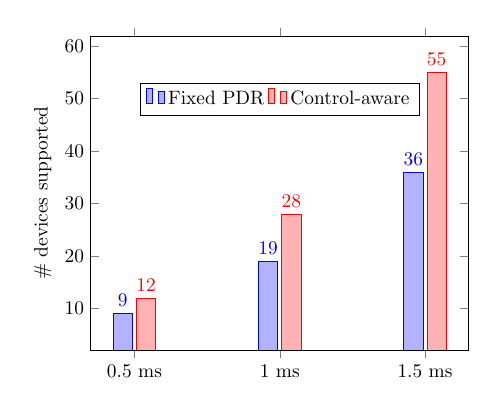
\begin{tikzpicture}[scale=0.7]
\begin{axis}[
    ybar,
    enlargelimits=0.15,
    legend style={at={(0.5,0.85)},
      anchor=north,legend columns=-1},
    ylabel={\# devices supported},
    symbolic x coords={0.5 ms,1 ms,1.5 ms},
    xtick=data,
    nodes near coords,
    nodes near coords align={vertical},
    ]
\addplot coordinates {(0.5 ms,9) (1 ms,19) (1.5 ms,36)};
\addplot coordinates {(0.5 ms,12) (1 ms,28) (1.5 ms,55)};
\legend{Fixed PDR, Control-aware}
\end{axis}
\end{tikzpicture} 
\caption{Simulation results for a series of inverted pendulums controlled over shared wireless channel. (left) The average distances from center vertical for $m=25$ pendulums. The control-aware, or ``co-design'', scheduler keeps all pendulums close, unlike the fixed PDR scheduler. (right) For different latency bounds, the control-aware can support more pendulums than the fixed PDR scheduler.}\label{fig_sim_results}
\end{figure*}


Given the set of devices selectively scheduled via \eqref{eq)prob_c}, we proceed to discuss an assignment-based formulation that can be employeed to select a low-latency schedule. Define the set of $m_k$ devices to selected be scheduled as $\ccalI_k \subseteq \{1,2,\hdots,m\}$ where  $| \ccalI_k| = m_k$ and device $j \in \ccalI_k$ with probability $\nu_{i,k}$. Further define $\ccalS_{(n)} \subset \ccalS$ to be an arbitrary set of $n$ FDs that do not intersect over any frequency bands, i.e. $\sum_{j \in \ccalS_{(n)}} \bbsigma_j \leq \mathbf{1}$. To accommodate the $m_k$ devices to be scheduled, we consider a set of $S$ such sets  $\{\ccalS^s_{(n_s)}\}_{s=1}^S$ with size $n_s$, whose combined elements total $\sum_{s=1}^{S} n_s = m_k$. We define this full set of assignable FDs at cycle $k$ as
%
\begin{align}\label{eq_ru_sets}
\ccalS'_k :=\ccalS^1_{(n_1)} \cup \ccalS^1_{(n_2)} \cup \hdots \cup \ccalS^{S_k}_{(n_{S_k})}.
\end{align}
%
Observe that an FD $\bbsigma$ is further superindexed by its TD slot $s$ y. In this way \eqref{eq_ru_sets} defines a complete set of  combinations of frequency-allocated FD and \emph{time}-allocated TDs to assign users during this cycle. An example of a possible $\ccalS'_k$ for scheduling $m_k = 12$ devices is shown in Table \ref{tab_rus}. 



For all $i \in \ccalI_k$ and FD $\bbsigma \in \ccalS'_k$, define the largest affordable DR given the \emph{modified} PDR requirement $\tdq_i(\hbx^{(l_i)}_{i,k})/\nu_{i,k}$ by
 %
 \begin{align}\label{eq_mcs_select}
 \mu_{i,k}(\bbsigma) := \begin{cases}
 \max \{\mu \mid q(\bbh_{i,k},\mu,\bbsigma) \geq \tdq_i(\hbx^{(l_i)}_{i,k})/\nu_{i,k}\} \\
 \mu_0,\quad  \text{ if } q(\bbh_{i,k},\mu,\bbsigma) < \tdq_i(\hbx^{(l_i)}_{i,k})/\nu_{i,k} \ \forall \mu
 \end{cases}
 \end{align}
 %
Observe in \eqref{eq_mcs_select} that, when no DR achieves the desired PDR in a particular FD, this value is set to $\mu=\mu_0$ by default.  The DR defined in \eqref{eq_mcs_select} subsequently incurs a time cost $\tau(\mu_{i,k}(\bbsigma), \bbsigma)$ for assigning device $i$ to FD $\bbsigma$. Define an \emph{assignment} $\ccalV=\{v_{ij}^s\}$ that assigns each device $i \in \ccalI_k$ to an FD/TD pair $(j,s)$ corresponding to an element in $\ccalS'_k$.  For time sensitive applications, the goal is to minimize the total transmission time across all TDs. The transmission time of a single TD is limited by the slowest device (i.e. a TD cannot finish until all devices finish transmitting). Thus, we can write the total transmission time as 
%
\begin{align}\label{eq_assignment}
T(\ccalV) = \sum_{s=1}^S \max_{j} \left[v^s_{ij} \tau(\mu_{i,k}(\bbsigma^s_j), \bbsigma_j^s)\right].
\end{align}
% 
The problem of minimizing $T(\ccalV)$ is a particular version of a non-linear assignment problem, where the goal is to choose an assignment---or schedule---that minimizes transmission time while meeting the control-aware PDR targets in \eqref{eq_pdr_constraint}. These problems are combinatorial in nature and challenging to solve exactly. We may approximate this problem by applying, e.g., the Hungarian method \cite{kuhn1955hungarian}, a well-known method for solving linear-cost assignment problems. Other heuristic assignment approaches may be designed to approximate the solution to \eqref{eq_assignment}. For the simulations performed later in this paper, we apply such a heuristic method, the details of which are left out for proprietary reasons.




The complete control-aware scheduling procedure for low-latency settings is present in Algorithm \ref{alg_calls}. At each cycle $k$, the BS uses current channel states $\bbh_{i,k}$ (obtained via pilot signals) and the current estimated control states $\hbx^{(l_i)}_{i,k}$  (obtained via \eqref{eq_state_est} for each device $i$) to compute control-aware target PDRs  $\tdq_i(\hbx^{(l_i)}_{i,k})$ for each device via \eqref{eq_pdr_constraint} in Step 3. In Step 4, the target PDRs are used to establish selection probabilities $\nu_{i,k}$ for each agent with \eqref{eq_prob_c}. After randomly selecting devices $\ccalI_k$ in Step 5, an appropriate set of FDs and TDs $\ccalS'_k$ are selected in Step 6. In Step 7, the associated DR values are determined for each possible assignment of device to FDs via \eqref{eq_mcs_select}. Finally, in Step 8 the assignment is performed using, e.g., the Hungarian method or other user-designed heuristic assignment method. The resulting assignment determines the scheduling parameters $\{\bbsigma_i, \mu_i, \alpha_i\}$ for all devices $i$ in the current cycle. 
 

%%%%%%%%%%%%%%%%%%%%%%%%%%%%%%%%%%%%%%%%%%%%%%%%%%%%%%%%%%%%%%%%%
%%%%%%%%%%%%%%%%%%%%%%%%%
%%%%%%% S E C T I O N %%%%%%%%%%%
%%%%%%%%%%%%%%%%%%%%%%%%%%
%%%%%%%%%%%%%%%%%%%%%%%%%%%%%%%%%%%%%%%%%%%%%%%%%%%%%%%%%%%%%%%%%%%%%
\section{Simulation Results}\label{sec_simulation}
In this section, we simulate the implementation of both the control-aware CALLS method and a standard ``control-agnostic'' scheduling methods for various low-latency control systems over a simulated wireless channel. We point out the low-latency based scheduling/assignment approaches of both methods being compared are identical, with the distinguishing features being the dynamic control-aware packet delivery rates incorporated in the CALLS method. In doing so, we may analyze the performance of the control-aware design outlined in the previous section relative to a standard latency-aware approach in terms of, e.g., number of users supported with fixed latency threshold or best latency achieved with fixed number of users. As we are interested primarily in low latency settings that tightly restrict the communication resources, we consider two standard control systems whose rapidly changing state requires high sampling rates, and consequently a communication latency on the order of milliseconds. The parameters for the simulation setup are provided in Table \ref{tab_simulation}. The packet delivery rate function $q(\bbh,\mu,\bbsigma)$ is computed using the standard AWGN noise curves for wireless channels. The transmission time $\tau(\mu,\bbsigma)$ is computed in the simulations using the associated data rates of an MCS in Table \ref{tab_mcs} for a 100 byte packet and overhead (e.g. TFs) of the 802.11ax specifications. The latency overhead for this setting amounts to approximately $\tau_0 \approx 100 \mu$s.
%
\begin{table}
\begin{tabular}{ l | l } \hline
  Channel model & IEEE Model E (indoor) \cite{liu2014ieee} \\
  Sensor to AP distances & Random (1 to 50 meters)\\
  Transmit power & 23 dbm \\
  Channel bandwidth & 20 MHz \\
  RU sizes & 2, 4, 8, 20 MHz \\
  \# of antennas at AP & 2 \\
  \# of antennas at sensors & 1 \\
  MCS options & See Table \ref{tab_mcs} \\
  State sampling period & 10 ms \\
  \hline
\end{tabular}
\caption{Simulation setting parameters.}
\label{tab_simulation}
\end{table}
%

\subsection{Inverted pendulum system}

\begin{figure}
\input{images/pendulum.tex}
\caption{Inverted pendulum-cart system $i$. The state $\bbx_{i,k} = [x_{i,k}, \dot{x}_{i,k}, \theta_{i,k}, \dot{\theta}_{i,k}]$ contains specifies angle $ \theta_{i,k}$ of the pendulum to the vertical, while the input $u_{i,k}$ reflects a horizontal force on the cart.}
\label{fig_inverted_pendulum}
\end{figure}


We perform an initial set of simulations on the well-studied problem of controlling a series of inverted pendulums on a horizontal cart. While conceptually simple, the highly unstable dynamics of the inverted pendulum make it a representative example of control system that requires fast control cycles, and subsequently low-latency communications when being controlled over a wireless medium. Consider a series of $m$ identical inverted pendulums, as pictured in Figure \ref{fig_inverted_pendulum}. Each pendulum of length $L$ is attached at one end to a cart that can move along a single, horizontal axis. The position of the pendulum changes by the effects of gravity and the force applied to the linear cart. For our experiments, we use the modeling of the inverted pendulum as provided by Quanser \cite{quanser}. The state is $p=4$ dimensional vector that maintains the position and velocity of the cart along the horizontal axis, and the angular position and velocity of the pendulum, i.e. $\bbx_{i,k} := [x_{i,k}, \dot{x}_{i,k}, \theta_{i,k}, \dot{\theta}_{i,k}]$. The system input $u_{i,k}$ reflects a horizontal force placed upon $i$th pendulum. By applying a zeroth order hold on the continuous dynamics with a state sampling rate of $0.01$ seconds and linearizing, we obtained the following discrete linear dynamic matrices of the pendulum system
%
\begin{align}\label{eq_control_orig}
\bbA_i =
\begin{bmatrix}
1 & 0 & 0 & 0 \\
0 & 2.055 & -0.722 & 4.828 \\
0 & 0.023 & 0.91 & 0.037 \\
0 & 0.677 & -0.453 & 2.055
\end{bmatrix},
\bbB_i =
\begin{bmatrix}
0.034 \\ 0.168 \\ 0.019 \\ 0.105
\end{bmatrix}.
\end{align}
%

Because the state $\bbx_{i,k}$ measures the angle of the $i$th pendulum at time $k$, the goal is to keep this close to zero, signifying that the pendulum remains upright. The input matrix $\bbK$ is computed to be a standard LQR-controller.

We perform a set of simulations scheduling the transmissions to control a series of inverted pendulums, varying both the latency threshold $\tau_{\max}$ and number of devices $m$. We perform the scheduling using the proposed CALLS method for control-aware low latency scheduling an, as a point of comparison, consider scheduling using a fixed ``high-reliability'' PDR of $0.99$ for all devices. Each simulation is run for a total of $1000$ seconds and is deemed ``successful'' if all pendulums remain upright for the entire run. We perform 100 such simulations for each combination of latency threshold and number of devices to determine how many devices we can support at each latency threshold using both the CALLS and fixed-PDR methods for scheduling.

In Figure \ref{fig_ip_dist} we show the results of a representative simulation of the control of $m=25$ pendulum systems with a latency bound of $\tau_{\max} = 10^{-3}$ seconds. In both graphs we show the average distance from the center vertical of each pendulum over the course of 1000 seconds. In the top figure, we see by using the control-aware CALLS method we are able to keep each of the 25 pendulums close to the vertical for the whole simulation. Meanwhile, using the standard fixed PDR, we are unable to meet the scheduling limitations imposed by the latency threshold, and many of the pendulums swing are unable to be kept upright, as signified by the large deviations from the origin. This is due to the fact that certain pendulums were not scheduled when most critical, and they subsequently became unstable.

%%%%
\begin{figure}
\centering
\includegraphics[width=.45\textwidth]{images/ip_dist.eps}
\caption{Average pendulum distance to center vertical for $m=25$ devices using (top) CALLS and (bottom) fixed-PDR scheduling with $\tau_{\max}= 1$ ms latency threshold. The proposed control aware scheme keeps all pendulums close to the vertical, while fixed-PDR scheduling cannot.}
\label{fig_ip_dist}
\end{figure}
%%

We present in Figure \ref{fig_ip_bar} the final capacity results obtained over all the simulations. We say that a scheduling method was able to successfully serve $m'$ devices if it keeps all devices within a  $|\theta_{i,k}| \leq 0.05$ error region for 100 independent simulations. Observe that the proposed approach is able to increase the number of devices supported in each case, with up to $1.5$ factor increase over the standard fixed PDR approach. Indeed, the proposed CALLS method is able to allocate the available resource in a more principled manner, which allows for the support of more devices simultaneously being controlled. 

%%%%%%
\begin{figure}
\centering
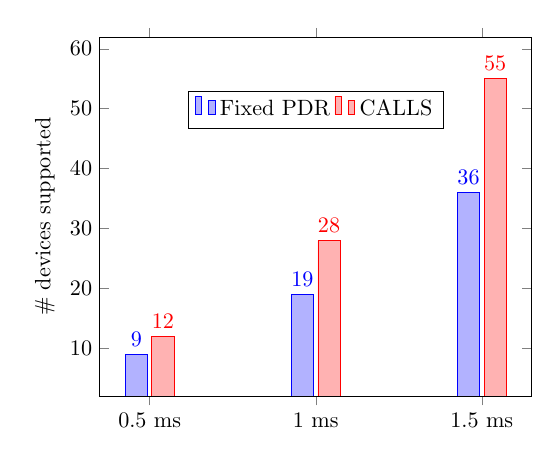
\begin{tikzpicture}[scale=0.8]
\begin{axis}[
    ybar,
    enlargelimits=0.15,
    legend style={at={(0.5,0.85)},
      anchor=north,legend columns=-1},
    ylabel={\# devices supported},
    symbolic x coords={0.5 ms,1 ms,1.5 ms},
    xtick=data,
    nodes near coords,
    nodes near coords align={vertical},
    ]
\addplot coordinates {(0.5 ms,9) (1 ms,19) (1.5 ms,36)};
\addplot coordinates {(0.5 ms,12) (1 ms,28) (1.5 ms,55)};
\legend{Fixed PDR, CALLS}
\end{axis}
\end{tikzpicture}
\caption{Total number of inverted pendulum devices that can be controlled using Fixed-PDR and CALLS scheduling for various latency thresholds.}
\label{fig_ip_bar}
\end{figure}
%%%%%%



\subsection{Balancing board ball system}

We perform another series of experiments on the wireless control of a series of balancing board ball systems developed by Acrome \cite{acrome}. In such a system, a ball is kept on a rectangular board with a single point of stability in the center of the board. Two servo motors underneath the board are used to push the board in the horizontal and vertical directions, with the objective to keep the ball close to the center of the board. The state here reflects the position and velocity in the horizontal and vertical axes, i.e. $\bbx_{i,k} := [x_{i,k}, \dot{x}_{i,k}, y_{i,k}, \dot{y}_{i,k}]$.  The input $\bbu_{i,k} = [v_x, v_y]$ reflects the voltage applied to the horizontal and vertical motors. As before, we apply a zeroth order hold on the continuous dynamics with a state sampling rate of $0.01$ seconds and linearize, thus obtaining the following dynamic system matrices,
%

\begin{align}\label{eq_control_orig}
\bbA_i =
\begin{bmatrix}
1 & 0.01 & 0 & 0 \\
0 & 1 & 0 & 0 \\
0 & 0 & 1 & 0.01 \\
0 & 0 & 0 & 1
\end{bmatrix},
\bbB_i =
\begin{bmatrix}
-0.0001 & 0\\ -0.02  & 0\\ 0 &-0.00008 \\ 0 & -0.01
\end{bmatrix}.
\end{align}
%
As before, we compute the control matrix $\bbK$ using standard LQR-control computation.

In Figure \ref{fig_bbb_dist} we show the results of a representative simulation of the control of $m=50$ balancing board ball systems with a latency bound of $\tau_{\max} = 10^{-3}$ seconds. Observe that, in this system, even with a large number of users the CALLS method can keep all systems very close to the center of the board, while the fixed PDR scheduler loses a few of the balls due to the agnosticism of the scheduler.

 To dive deeper into the benefits provided by control aware scheduling, we present in Figure \ref{fig_bbb_psr} a histogram of the actual  packet delivery rates each of the devices achieved over the representative simulation. It is interesting to observe that, in the CALLS method, the achieved PDRs are closely concentrated, ranging from 0.3 to 0.44. On the other hand, using a fixed PDR scheduling scheme, the non-variable rates are too strict for the low-latency system to support, and without control-aware scheduling the achieved PDRs range wildly from close to 0 to close to 1. In this case, some devices are able to transmit almost every cycle while others are almost never able to successfully transmit their packets. This suggests that, by using control aware scheduling, we indirectly achieve a sense of fairness across users over the long term. Further note that the PDRs required to keep the balancing board ball stable, e.g. 0.4, are relatively small. This is due to the fact that the balancing board ball features relatively slow moving dynamics, making it easier to control with less frequent transmissions. This is comparison to the inverted pendulum system, in which the pendulums were kept stable with PDRs in the range 0.6-0.75.

%%%%
\begin{figure}
\centering
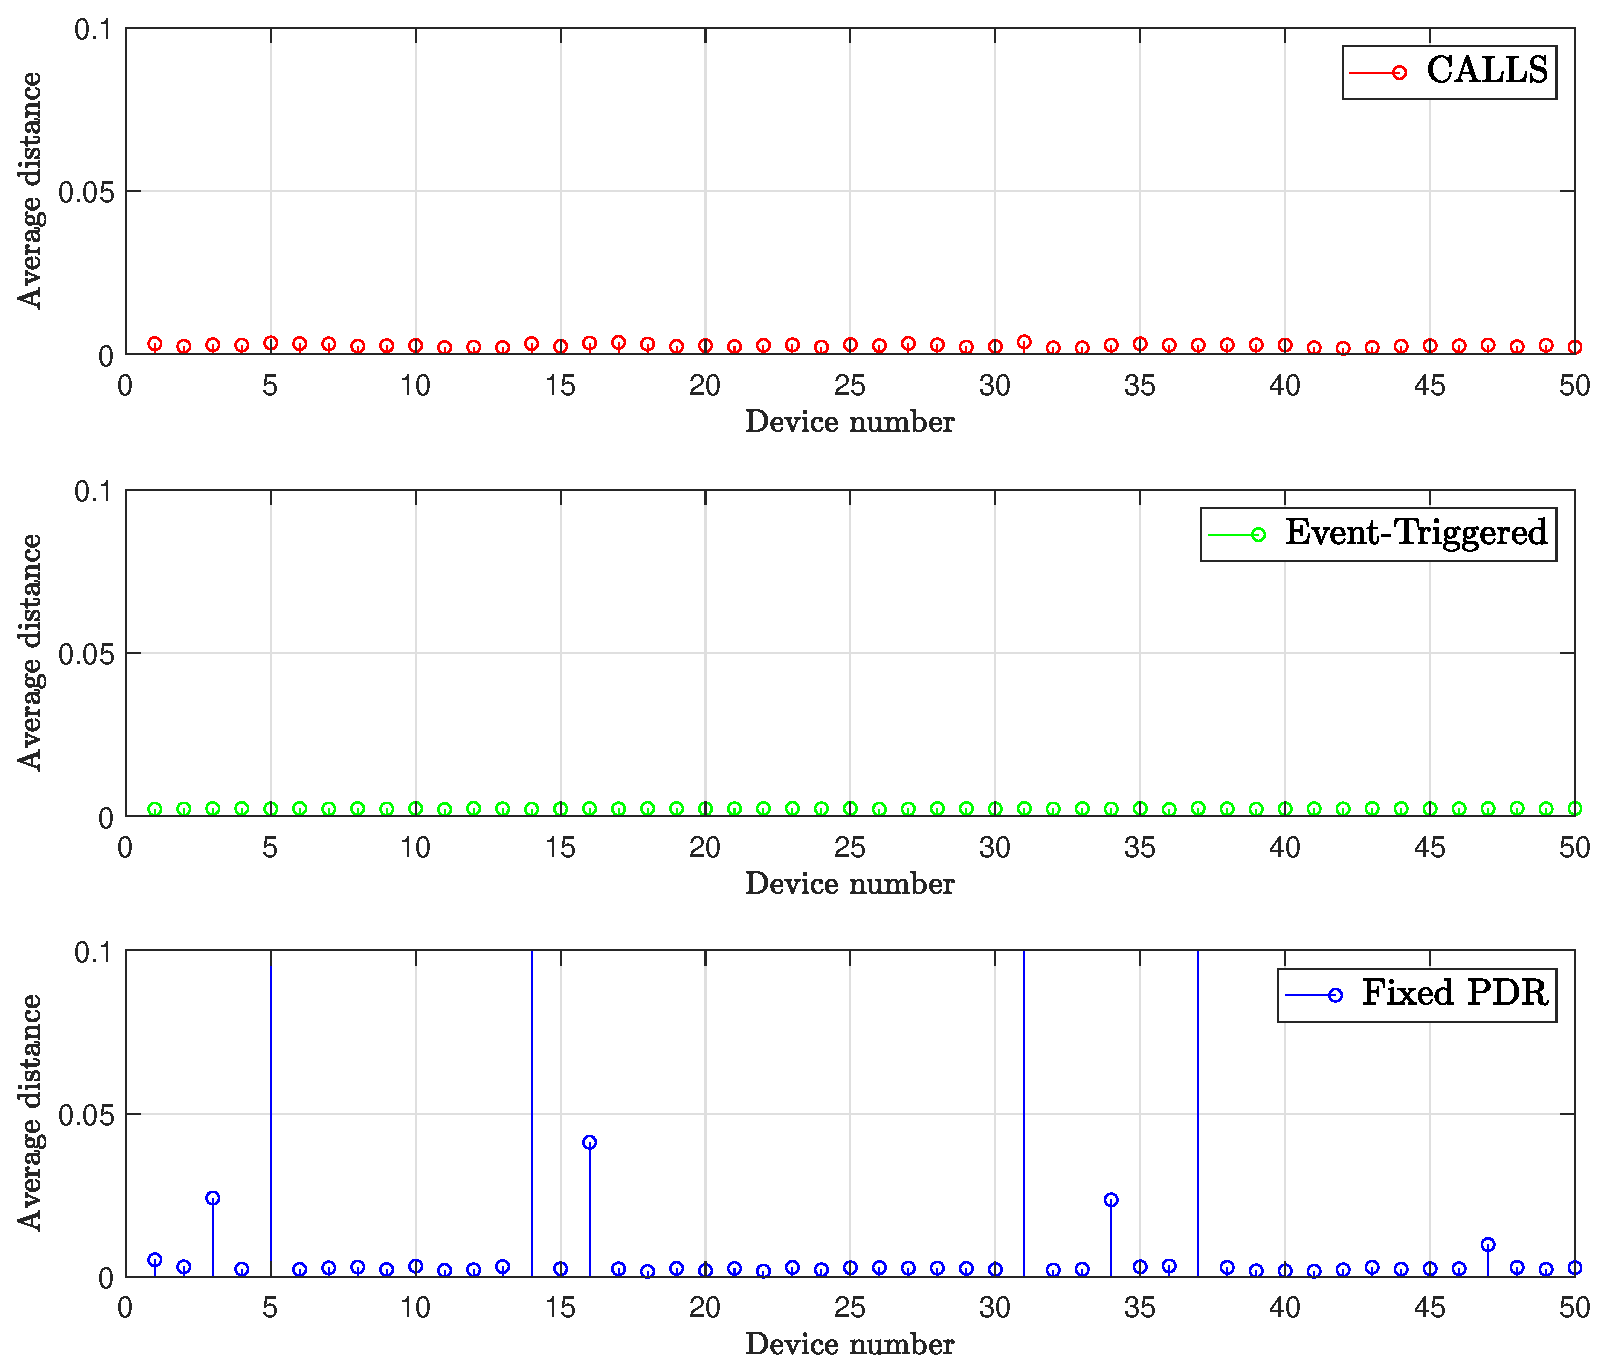
\includegraphics[width=.45\textwidth]{images/bbb_dist.eps}
\caption{Average ball distance to center for $m=50$ devices using (top) CALLS and (bottom) fixed-PDR scheduling with $\tau_{\max} =1$ ms latency threshold. The proposed control aware scheme keeps all balancing balls close to center, while fixed-PDR scheduling cannot.}
\label{fig_bbb_dist}
\end{figure}
%%

%%%%
\begin{figure}
\centering
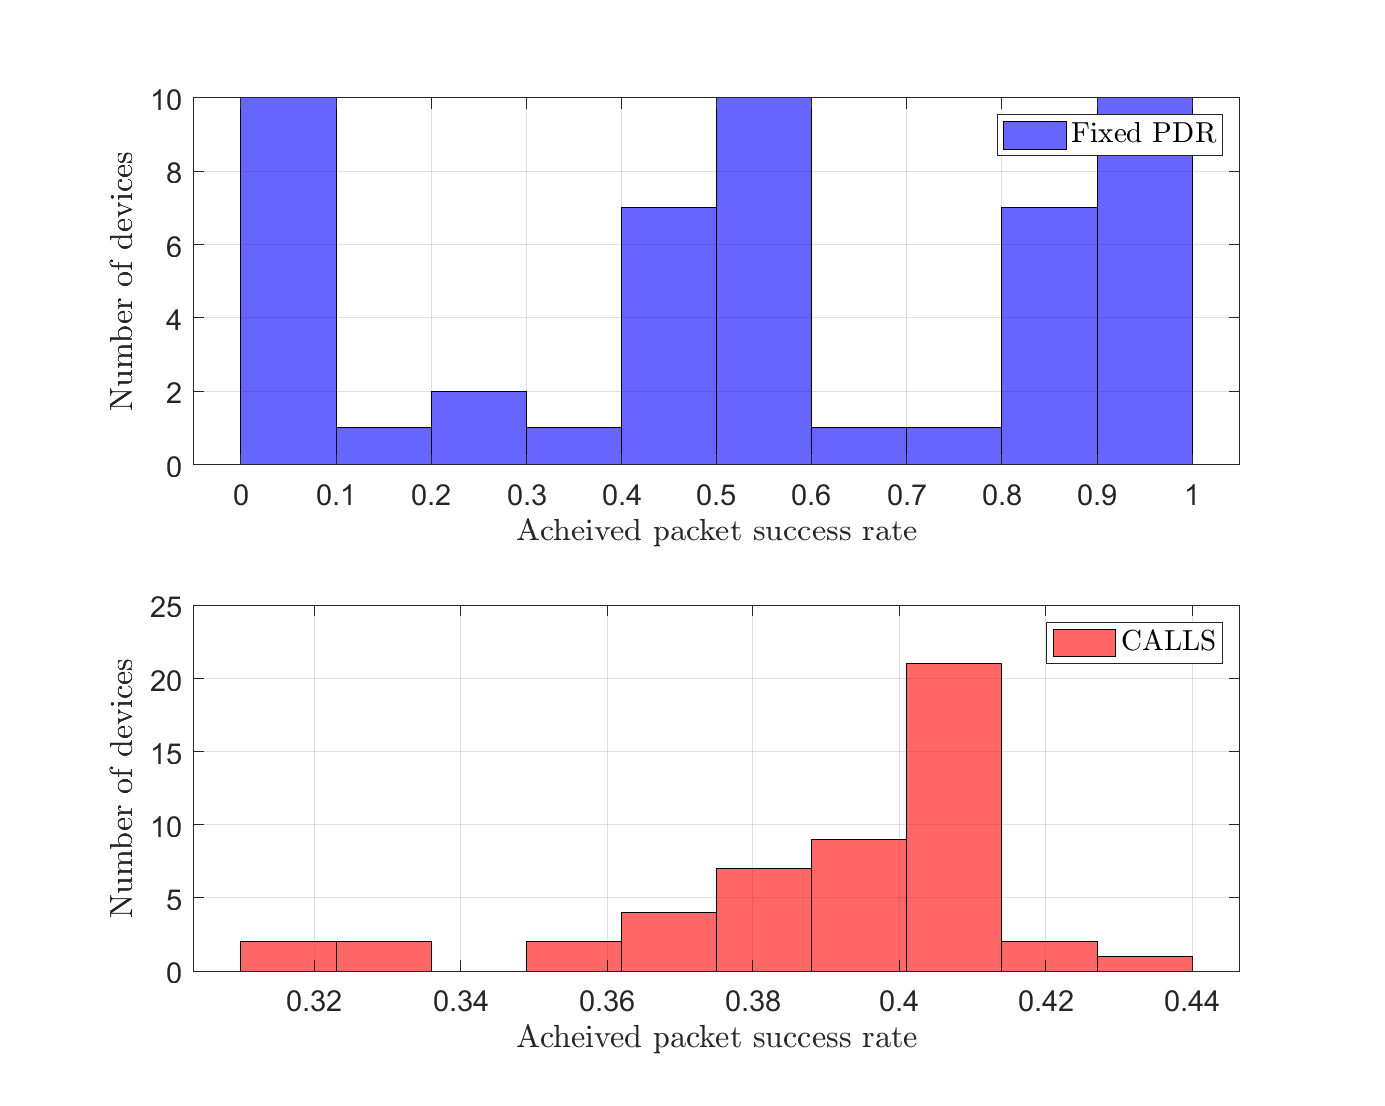
\includegraphics[width=.45\textwidth]{images/bbb_psr.eps}
\caption{Histogram of achieved PDRs in $m=50$ balancing board systems (top) CALLS and (bottom) fixed-PDR scheduling with $\tau_{\max} =1$ ms latency threshold. The proposed control aware scheme achieves similar PDRs for all devices, while the control agnostic scheduling results in large variation in packet delivery.}
\label{fig_bbb_psr}
\end{figure}
%%

We present in Figure \ref{fig_bbb_bar} the final capacity results obtained over all the simulations for the balancing board ball system. Observe that proposed approach increases the number of supported devices by factor of 2 relative to the standard fixed PDR approach. The even greater improvement here relative to the inverted pendulum simulations can be attributed to the slower dynamics of the balancing board ball, which allows for even more gains using control-aware PDRs due to the lower PDR requirements of the system.


%%%%%%
\begin{figure}
\centering
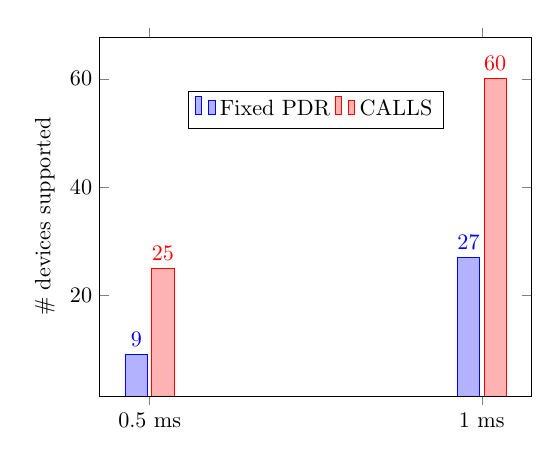
\begin{tikzpicture}[scale=0.8]
\begin{axis}[
    ybar,
    enlargelimits=0.15,
    legend style={at={(0.5,0.85)},
      anchor=north,legend columns=-1},
    ylabel={\# devices supported},
    symbolic x coords={0.5 ms,1 ms},
    xtick=data,
    nodes near coords,
    nodes near coords align={vertical},
    ]
\addplot coordinates {(0.5 ms,9) (1 ms,27)};
\addplot coordinates {(0.5 ms,25) (1 ms,60)};
\legend{Fixed PDR, CALLS}
\end{axis}
\end{tikzpicture}
\caption{Total number of balancing ball board devices that can be controlled using Fixed-PDR and CALLS scheduling for various latency thresholds.}
\label{fig_bbb_bar}
\end{figure}
%%%%%%




%%%%%%%%%%%%%%%%%%%%%%%%%%%%%%%%%%%%%%%%%%%%%%%%%%%%%%%%%%%%%%%%%
%%%%%%%%%%%%%%%%%%%%%%%%%
%%%%%%% S E C T I O N %%%%%%%%%%%
%%%%%%%%%%%%%%%%%%%%%%%%%%
%%%%%%%%%%%%%%%%%%%%%%%%%%%%%%%%%%%%%%%%%%%%%%%%%%%%%%%%%%%%%%%%%%%%%
\section{Discussion and Conclusions}\label{sec_conclusion}
In this paper we proposed a novel control-communication co-design approach to solving the radio resource
allocation problem for time-sensitive wireless control systems. Given a channel state and control state, we mathematically derive a minimum packet delivery
rate a device must meet to maintain a control-orientated target,
as defined by a stability-inducing Lyapunov function. By
dynamically assigning variable packet delivery rate targets
to each device based on its current conditions, we are able to
more easily meet feasibility requirements of a latency-constrained
wireless control problem and maintain stability
and strong performance. We perform simulations on numerous
well-studied low-latency control problems to demonstrate the
benefits of using the control-aware approach, which can include
a 2x gain on number of devices that can be supported.

The results presented in this paper suggest an interesting
potential for control-aware resource allocation and scheduling, particularly in low-latency industrial systems. By considering the control-specific targets such as maintaining
stability or an error margin, we observe that the standard
high reliability targets considered (e.g. packet delivery rates $\geq 0.999$) can in some cases be substantially stricter than
necessary for adequate performance. Wireless control systems
with sufficiently slow dynamics can be kept stable with much
lower packet delivery rates, which in turn make low-latency
communications more achievable. Furthermore, in realistic industrial systems there will be many heterogeneous devices being controlled, whose variation in communication needs is well-served by control-aware opportunism proposed in this paper. This suggests the potential for wireless communications to be adopted using a smart control-communication co-design approach even
while ultra-reliable wireless system technology remains under development.



% References should be produced using the bibtex program from suitable
% BiBTeX files (here: strings, refs, manuals). The IEEEbib.bst bibliography
% style file from IEEE produces unsorted bibliography list.
% -------------------------------------------------------------------------
\urlstyle{same}
\bibliographystyle{IEEEtran}
\bibliography{../wireless_ll_control,../scheduling_control}


\end{document} 